\begin{center}
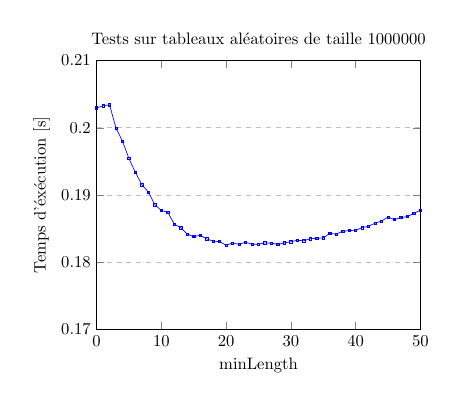
\begin{tikzpicture}[scale=0.6]
\begin{axis}[
    title={Tests sur tableaux aléatoires de taille $1 000 000$},
    xlabel={minLength},
    ylabel={Temps d'éxécution [s]},
    xmin=0, xmax=50,
    ymin=0.17,ymax=0.21,
    xtick={0,10,20,30,40,50},
    ytick={0.17,0.18,0.19,0.20,0.21},
    legend pos=north west,
    ymajorgrids=true,
    grid style=dashed,
]
 
\addplot[
    color=blue,
	mark=square,
	mark size=0.7
    ]
    coordinates {
    (0,0.202960)(1,0.203280)(2,0.203410)(3,0.199960)(4,0.198010)(5,0.195420)(6,0.193360)(7,0.191530)(8,0.190440)(9,0.188560)(10,0.187710)(11,0.187440)(12,0.185680)(13,0.185140)(14,0.184200)(15,0.183820)(16,0.184020)(17,0.183480)(18,0.183140)(19,0.183080)(20,0.182550)(21,0.182860)(22,0.182680)(23,0.182990)(24,0.182690)(25,0.182700)(26,0.182890)(27,0.182860)(28,0.182660)(29,0.182900)(30,0.183060)(31,0.183280)(32,0.183200)(33,0.183500)(34,0.183570)(35,0.183620)(36,0.184300)(37,0.184180)(38,0.184620)(39,0.184720)(40,0.184770)(41,0.185150)(42,0.185370)(43,0.185820)(44,0.186130)(45,0.186730)(46,0.186350)(47,0.186650)(48,0.186810)(49,0.187270)(50,0.187770) 
	};
 
\end{axis}
\end{tikzpicture}
\end{center}
